\chapter{Related Work}

\section{Frameworks}
Many mature frameworks exist to implement CNNs on CPU and GPU computing platforms. For FPGA, frameworks are still relatively elementary. Lui et al. \cite{liu2016automatic} implements a Verilog source code generator using a domain-specific language consisting of tuples of parameters describing each layer in a CNN configuration. Each layer is capable of being analytically modeled to estimate computation complexity, execution time, and resource usage based on their input parameters. For compute, they use the convolver CCU, which is a pipelined convolutional kernel with data reuse via registers. Guo et al. \cite{guo2018angel} implements Angel-Eye, a complete design flow for mapping CNNs onto FPGAs. They first collect statistics on the feature maps and network parameters to get a histogram of their logarithm value, which inspires how they can choose the radix point for fixed point floats layer by layer. For their CCU, they adopt a 3x3 convolution kernel based on the reconfigurable line buffer design \cite{zhang2016caffeine} that supports any kernel size. Data is arranged as row-major tiles. They require a single row in a tile to have enough elements to maximize the DRAM burst length. The number of rows in a single tile is chosen by a set of rules that minimizing DRAM memory accesses. DiCecco et al. \cite{dicecco2016caffeinated} implements Caffeinated, a modification of Caffe for FPGA support alongside a host processor. The FPGA is used as a dedicated accelerator for 3x3 convolution layers using a Winograd-based CCU. Lu et al. \cite{lu2017evaluating} implements another Winograd- based approach with code generation. They too employ a line buffer structure similar to Angel- Eye. They model their resource usages which is used to maximize Winograd CCU parallelism within a given FPGA, and generate respective HLS code. Tu et al. \cite{tu2017deep} implements Deep Neural Architecture (DNA), an acceleration architecture chip with reconfigurable computation patterns for different models. DNA reconfigures its data path to maximize data reuse based on the model to minimize energy usage. Data reuse is accomplished by tiling input and output feature maps with different configurations per layer that minimize off-chip memory accesses. While DNA is not designed for FPGAs, many of its hardware optimizations can be considered in FPGA implementations.

\section{Convolution Computation Units}
\subsection{Convolver}
The convolver \cite{liu2016automatic} exploits pipelined parallelism by using a sliding window when scanning a single channel, and is connected to a reduction tree to get a single output element per cycle. Convolvers are fixed to the size of a kernel. It is assumed feature maps are stored row-wise for coalesced data accesses to feed the convolver.

Their experimental results only consider two sequential models, AlexNet \cite{krizhevsky2012imagenet} and LeNet \cite{lecun1998gradient}. Their FPGA is large enough to map each layer onto the FPGA. Within AlexNet are kernel sizes of 11x11, 7x7, and 3x3. Three independent convolvers of each size are needed to support all convolution layers. In the case where FPGA resources are limited, there may not be enough DSPs to account for all CCUs. Alternatively, when there are sufficient resources for each CCU, each one needs a sufficient memory buffer to avoid stalling. Otherwise, bottlenecks will occur in the pipeline, causing convolvers to not be fully utilized. They do not elaborate on how their framework can be used to mitigate this problem. Lastly, the convolver is not optimal for convolutions with stride greater than one. The computation is not coalesced, and requires overhead to orchestrate either the data access pattern or convolver input, both of which can also stall the pipeline.

\begin{figure}
		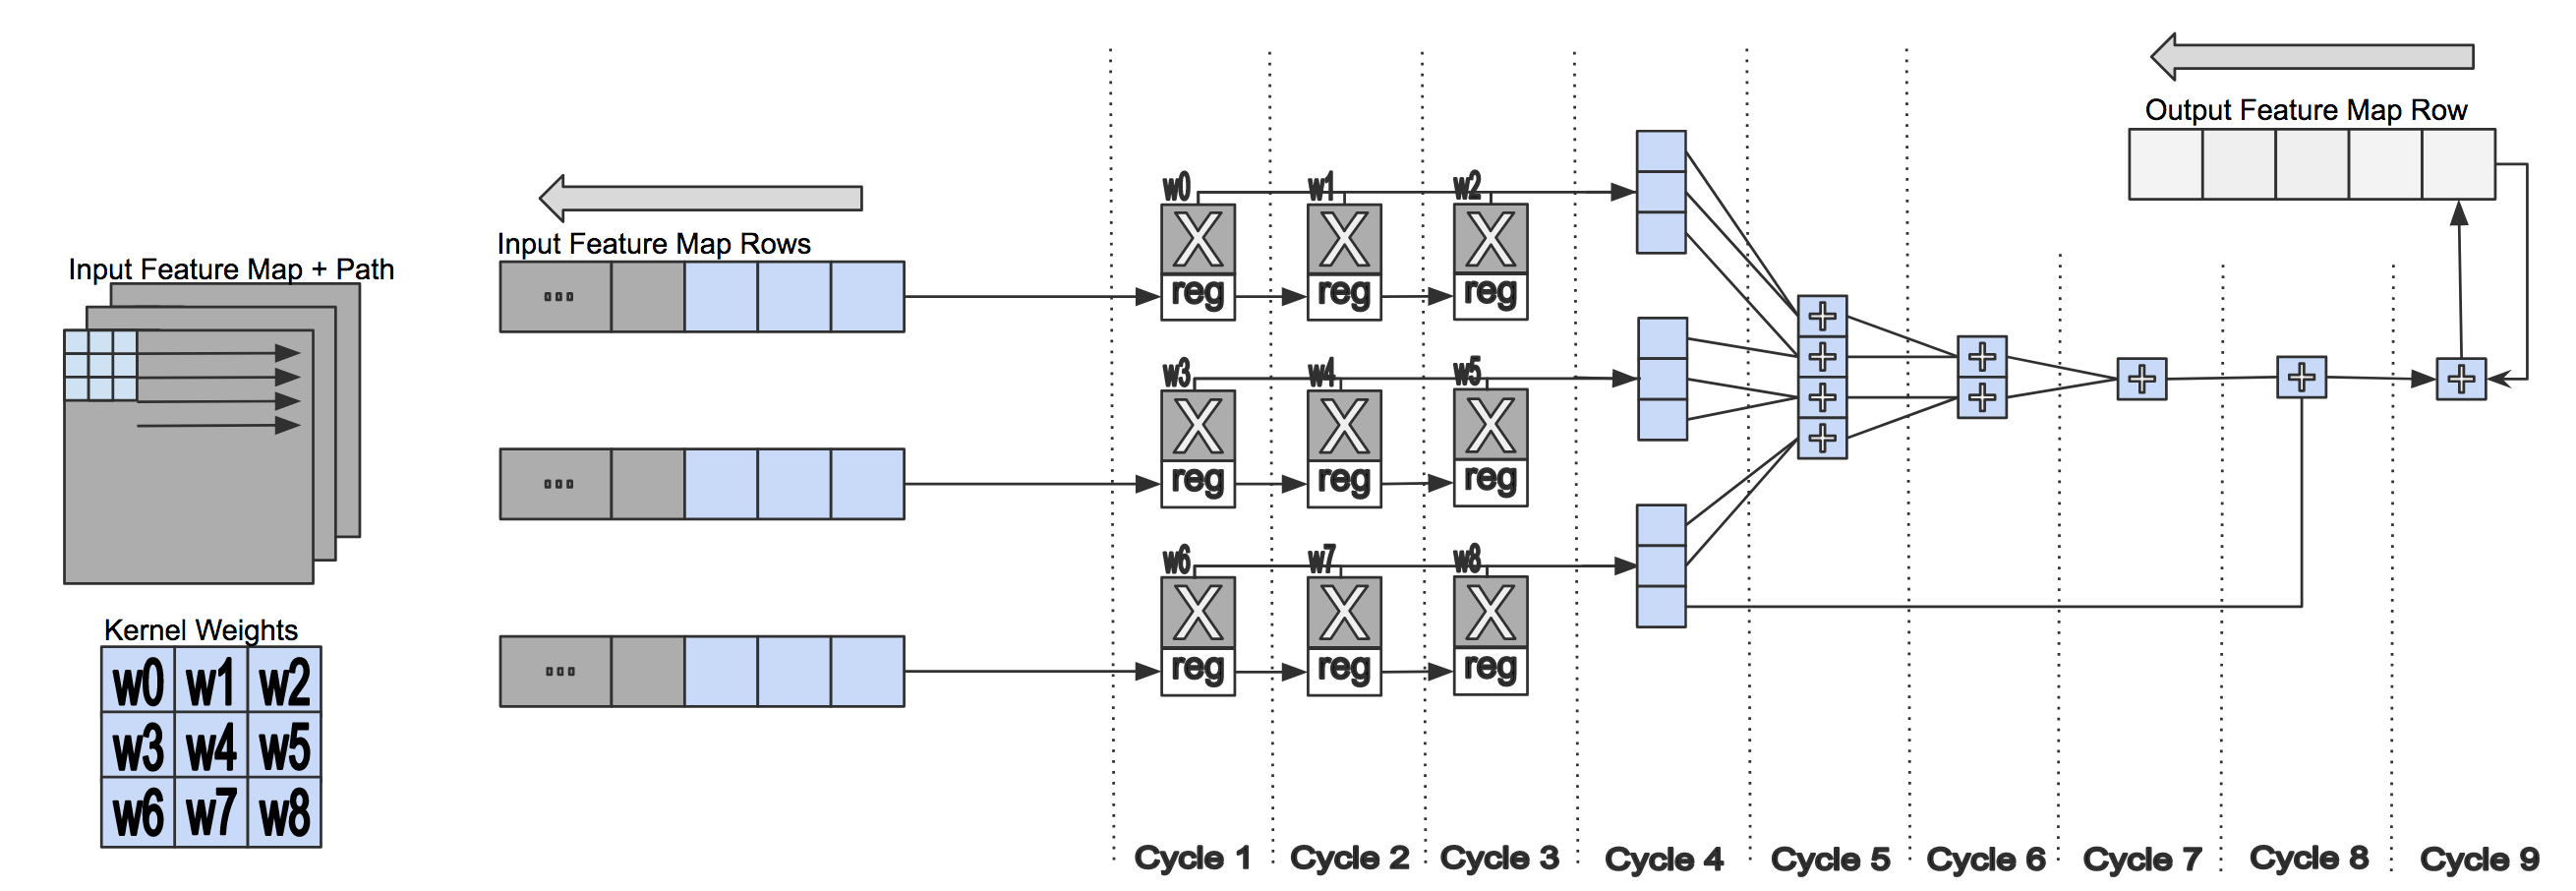
\includegraphics[scale=0.35]{ConvolverDiagram}
		\caption[Convolver Diagram]%
		{\narrower Convolver with a 3x3 kernel. Loads three rows into RAM and performs a sliding window to load values into registers and compute the convolution.}
		\label{control-file}
\end{figure}

\subsection{Output Oriented Mapping}
Previous works consider Output Oriented Mapping (OOM) \cite{zhang2015optimizing, chen2017eyeriss, rahman2016efficient}, which loads an input map into its CCU and performs convolution using a single weight in all processing elements (PEs). Both OOM and convolver exploit data reusability via sliding window interconnects between PE registers. The benefit of OOM is it can support various kernel sizes with a fixed number of DSPs without having to allocate k-by-k DSPs for each weight in a kernel. However, OOM too suffers from stride greater than one for the same reasons as convolver.

\subsection{Parallel OOM}
DNA from \cite{tu2017deep} extends OOM using parallel (POOM), a modification that parallel computes P feature maps on the PE array. In the example above, if stride were equal to two, the PE array’s middle column would be unutilized. POOM will use that column to compute the convolution of an additional feature map.

\subsection{Winograd CCU}
Winograd convolution \cite{winograd1980arithmetic} has been used to accelerate convolutions of small kernels in other CNN implementations \cite{dicecco2016caffeinated, lavin2016fast, lu2017evaluating}. It is an algorithm that exploits the multiplicative structure of FFT and transforms it into a cyclic convolution computation \cite{winograd1976computing}. The end result is a convolution algorithm that requires less multiplications and more additions via matrix multiplications (GEMMs). Most hardware platforms, including FPGAs, contain optimizations specifically for GEMM. The Winograd convolution exploits this to accelerate convolution computation. Winograd output is referred to as F(mxm, rxr), where mxm represents the number of output values and rxr is the filter size. \cite{dicecco2016caffeinated} implements a F(2x2, 3x3) Winograd CCU with unity stride. An output size of 2x2 with 3x3 kernels requires 4x4 input size. Feature maps are tiled using 4x2 blocks with replicated values in the rows to store overlapping data in successive Winograd convolutions along a column. The tile width of two results in no overlaps in Winograd convolutions along a row. Tiles are fed into the CCU row-wise and compute partial outputs. Partial outputs of the transformed data are computed in parallel along multiple columns of a row, allowing successive reuse for neighboring tiles. Following that, each 4x2 tile and its neighboring tile are fed into a pipelined CU that handles all subsequent computations after the initial transformation.

\section{Memory Access Patterns}
\subsection{Row/Column Major}
The most basic form of storing kernel weights and input/output feature maps is depth x row x column or depth x column x row, such that columns or rows are operated on first. For the convolver and OOM-like CCUs, they can be feed rows of data that reuse adjacent columns within registers. Several memory access penalties can occur if multiples rows cannot be stored in BRAM. If a row is sufficiently large, multiple data accesses to DRAM must be made on successive rows. Additionally, DRAM access can only exploit burst-mode for a single row of data. When accessing a subset of multiple rows, each row within the subset is not contiguous, causing additional memory requests for each row.

\subsection{Tiling}
Many CNN-FPGA implementations tile data to avoid the pitfalls of row or column major formatting \cite{tu2017deep, dicecco2016caffeinated, bettoni2017convolutional, guo2018angel}. Tiles often contain duplicated data in their overlapped regions such that a single tile is only ever accessed once during layer computation. It is typical to only tile the feature maps and not the channels, such that multiple CCUs can operate on independent channels in parallel. Tile sizes are often chosen with respect to data burst lengths, kernel sizes, number of channels, and BRAM buffer sizes for inputs, outputs, and weights.